
\begin{figure*}[t]
\centering
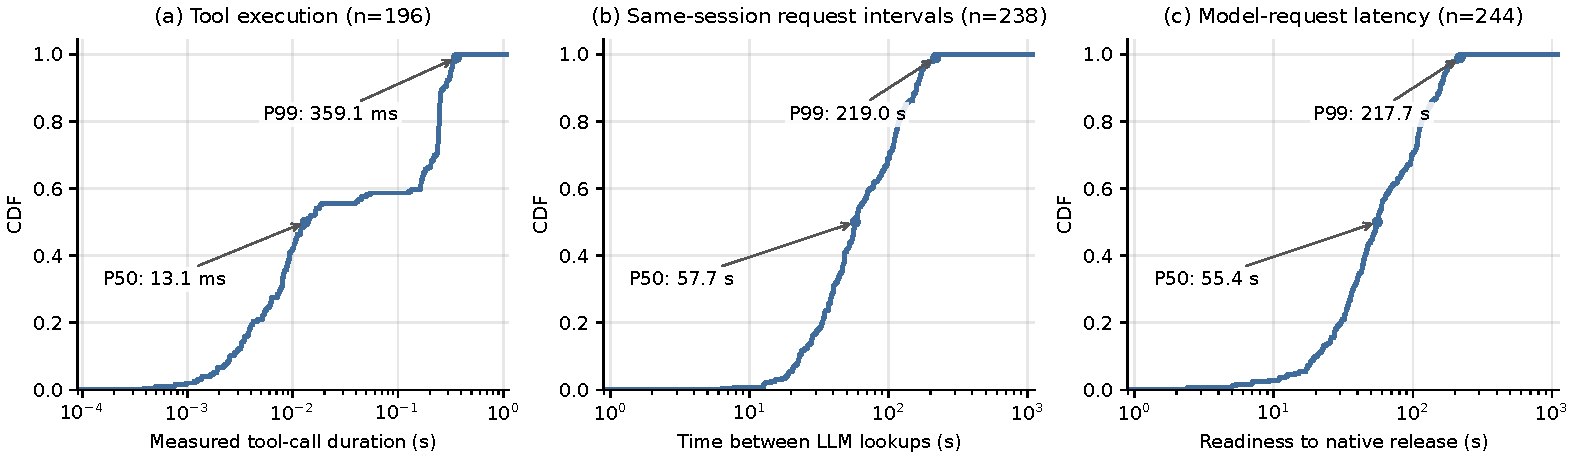
\includegraphics[width=\textwidth]{leasepath_isca_v3_assets/figures/workload_request_durations.pdf}
\caption{Tool execution is brief, while request intervals and latency span much longer timescales; markers show empirical P50/P99.}
\Description{Three logarithmic CDFs separately show actual tool execution,
same-session lookup-to-lookup intervals, and request readiness-to-release
latency, with median and 99th-percentile annotations.}
\label{fig:request-durations}
\end{figure*}

Figure~\ref{fig:request-durations} summarizes tool and request timing
with logarithmic empirical CDFs. Measured tool execution has P50
13.1 ms and P99 359.1 ms (196 calls). For each project,
the interval between successive native lookup starts has P50
57.715 seconds and P99 219.031 seconds (238 pairs). This interval
includes the preceding model execution and the subsequent tool/user,
controller, and queue delays; it differs from the release-to-lookup
idle interval discussed below.

Per-model-request latency is measured from recorded readiness to native
release: P50 55.354 seconds and P99 217.705 seconds (244 requests).
It includes notification handling, FCFS waiting, preparation, and model
service, rather than only GPU execution. It also differs from the
validated user-turn response, which can span multiple model requests
and tools. These descriptive percentiles concern six correlated
development histories, not independent tail-latency estimates.
